\documentclass[tikz]{standalone}

\usepackage{tikz}
\usetikzlibrary{positioning,shapes,backgrounds}
\usepackage{tkz-euclide}

\begin{document}

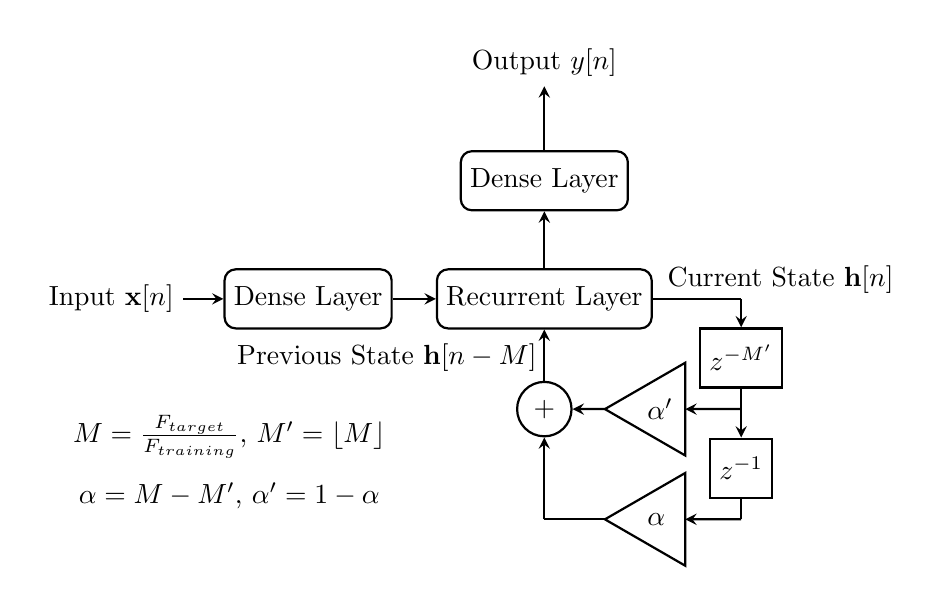
\begin{tikzpicture}[node distance=1.5cm, background rectangle/.style={fill=white}, show background rectangle]
    \tikzset{
        mynode/.style = {rectangle, rounded corners, line width=0.8pt, minimum width=1.0cm, minimum height=0.75cm, text centered, draw=black, fill=white},
        amp/.style = {regular polygon, regular polygon sides=3, draw, fill=white, text width=0.8em,
                      inner sep=1mm, outer sep=0mm, shape border rotate=90, line width=0.8pt},
        arrow/.style = {thick,->,>=stealth},
        delay/.style = {rectangle, draw=black, line width=0.8pt, minimum height=0.75cm}
    }
    \node (input) {Input $\mathbf{x}[n]$};
    \node (dlayer) [mynode, right of=input, xshift=1.0cm] {Dense Layer};
    \node (rlayer) [mynode, right of=dlayer, xshift=1.5cm] {Recurrent Layer};
    \coordinate[right of=rlayer, xshift=1.0cm] (h0) ;
    \node (h0Label) [right of=h0, yshift=0.25cm, xshift=-1cm] {Current State $\mathbf{h}[n]$};

    \node (zM) [delay, below of=h0, yshift=0.75cm] {$z^{-M'}$};
    \coordinate[below of=zM, yshift=0.85cm] (hM);
    \node (gM) [amp, left of=hM, xshift=0.45cm] {$\alpha'$};
    \node (sum) [draw, fill=white, circle, line width=0.8pt, below of=rlayer, yshift=0.1cm] {+};


    \node (z1) [delay, below of=hM, yshift=0.75cm] {$z^{-1}$};
    \coordinate[below of=z1, yshift=0.85cm] (h1);
    \node (g1) [amp, left of=h1, xshift=0.45cm] {$\alpha$};
    \coordinate[below of=sum, yshift=0.1cm] (hSum);

    \draw [arrow] (input) -- (dlayer);
    \draw [arrow] (dlayer) -- (rlayer);
    \draw [thick] (rlayer) -- (h0);

    \draw [arrow] (h0) -- (zM);
    \draw [thick] (zM) -- (hM);
    \draw [arrow] (hM) -- (gM);
    \draw [arrow] (gM) -- (sum);

    \draw [arrow] (hM) -- (z1);
    \draw [thick] (z1) -- (h1);
    \draw [arrow] (h1) -- (g1);
    \draw [thick] (g1) -- (hSum);
    \draw [arrow] (hSum) -- (sum);

    \draw [arrow] (sum) -- (rlayer);

    \node (dense) [mynode, above of=rlayer] {Dense Layer};
    \node (out) [above of=dense] {Output $y[n]$};
    \draw [arrow] (rlayer) -- (dense);
    \draw [arrow] (dense) -- (out);

    \node (h1Label) [below of=rlayer, yshift=0.75cm, xshift=-2.0cm] {Previous State $\mathbf{h}[n-M]$};
    \node (MLabel) [below of=dlayer, yshift=-0.25cm, xshift=-1cm] {$M = \frac{F_{target}}{F_{training}}$, $M' = \lfloor M \rfloor$};
    \node (alphaLabel) [below of=MLabel, yshift=0.75cm] {$\alpha = M - M'$, $\alpha' = 1 - \alpha$};
\end{tikzpicture}

\end{document}
